\documentclass[12pt,a4paper]{exam}

% --------------------
% Packages
% --------------------
\usepackage[utf8]{inputenc}
\usepackage[T1]{fontenc}
\usepackage[french]{babel}
\usepackage{mdframed}
\usepackage{amsmath,amssymb}
\usepackage{xcolor}
\usepackage[dvipsnames]{xcolor}
\usepackage{multicol}
\usepackage{geometry}
\usepackage{graphicx}

\setlength{\parindent}{0pt}

\geometry{margin=2cm}

% --------------------
% En-tête / pied
% --------------------
\header{}{}{2nde générale}
\footer{}{\thepage}{\it{G.M.}}

% --------------------
% \renewcommand{\questionlabel}{\alph{question})}
\begin{document}

\begin{center}
    \Large\textbf{\underline{DM : vers la 1ère}\\Nombre dérivé}
\end{center}

\vspace{5pt}

% ======================================================
\noindent
\textbf{Exercice 1 : Vers le nombre dérivé}

\vspace{10pt}
\begin{minipage}[t]{.55\textwidth}%
    \vspace{5pt}
    \hspace{0.5cm} Soit $f$ la fonction définie sur $\mathbb{R}$ par $f(x) = x^2$. 
On appelle $\mathcal{C}_f$, sa courbe représentative dans un repère orthonormé et 
on considère le point $A$ de $\mathcal{C}_f$, d'abscisse 2.

\vspace{5pt}
Soit $h$ un réel non nul. On appelle $H$ le point de $\mathcal{C}_f$, d'abscisse $2+h$.

\vspace{5pt}
On s'intéresse aux coefficients directeurs des droites $(AH)$ quand $h$ se rapproche de $0$.

\vspace{5pt}
On note $\tau(h)$ le coefficient directeur de la sécante $(AH)$.
\end{minipage}%
\hfill
\begin{minipage}[t]{.35\textwidth}%
    \vspace{-30pt}
    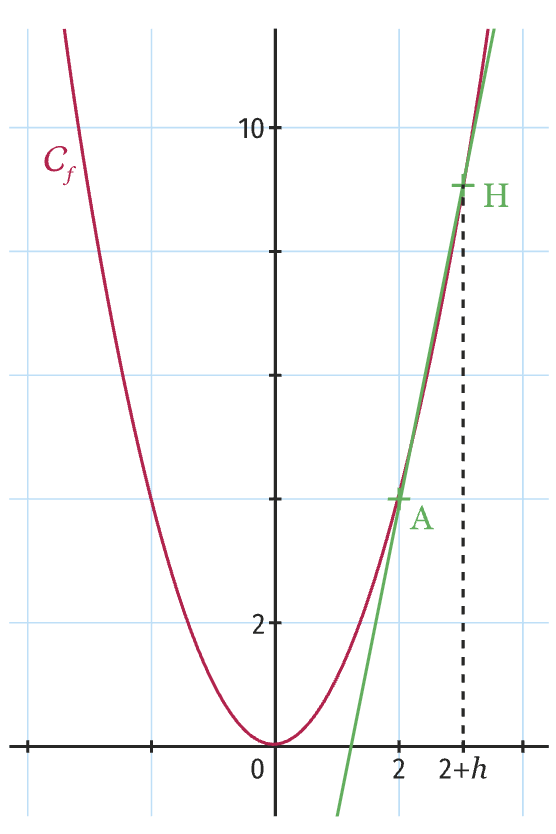
\includegraphics[width=0.85\textwidth]{graphic.png}
\end{minipage}%

\vspace{10pt}
\begin{questions}
    \question En faisant des calculs à la main, relever les valeurs 
    des coefficients directeurs des droites sécantes $(AH)$ à $\mathcal{C}_f$ pour 
    les différentes valeurs de $h$ données dans ce tableau :
    
    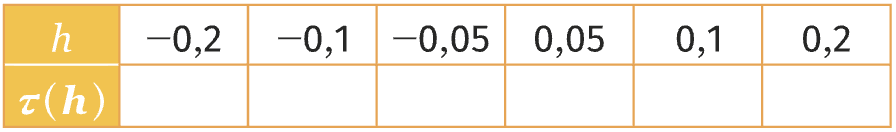
\includegraphics[width=0.55\textwidth]{tableau.png}

    \vspace{5pt}
    \question Quand $h$ prend des valeurs de plus en plus proches de $0$,
    vers quel point de la courbe $\mathcal{C}_f$ le point $H$ semble-t-il se 
    rapprocher ?
    \\De quelle valeur le coefficient directeur $\tau(h)$ semble-t-il se 
    rapprocher ?

    \vspace{5pt}
    \question Exprimer en fonction de $h$ le coefficient directeur $\tau(h)$ de la droite 
    $(AH)$ lorsque $A$ et $H$ sont \textbf{distincts}.
\vspace{5pt}
\end{questions}

\vspace{10pt}

% ======================================================
\noindent
\textbf{Exercice 2 : Définition et dérivabilité}

\begin{minipage}[t]{.55\textwidth}%
    \vspace{5pt}
    \hspace{0.5cm}Le nombre $\tau(h) = \dfrac{f(a+h)-f(a)}{h}$ 
est appelé
\textbf{taux de variation} de $f$ entre $a$ et $a+h$. 

\vspace{15pt}
Sur la figure ci-contre, 
le point $A$ a pour coordonnées $(a; f(a))$ et le point $H$ a pour 
coordonnées $(a+h; f(a+h))$.

\vspace{15pt}
Le coefficient directeur de la droite $(AH)$ est 
$\dfrac{f(a+h)-f(a)}{a+h-a}$ ; autrement dit, le coefficient 
directeur est $\tau(h)$.
\\Le nombre $\tau(h)$ dépend de $a$.
\end{minipage}%
\hfill
\begin{minipage}[t]{.4\textwidth}%
    \vspace{0pt}
    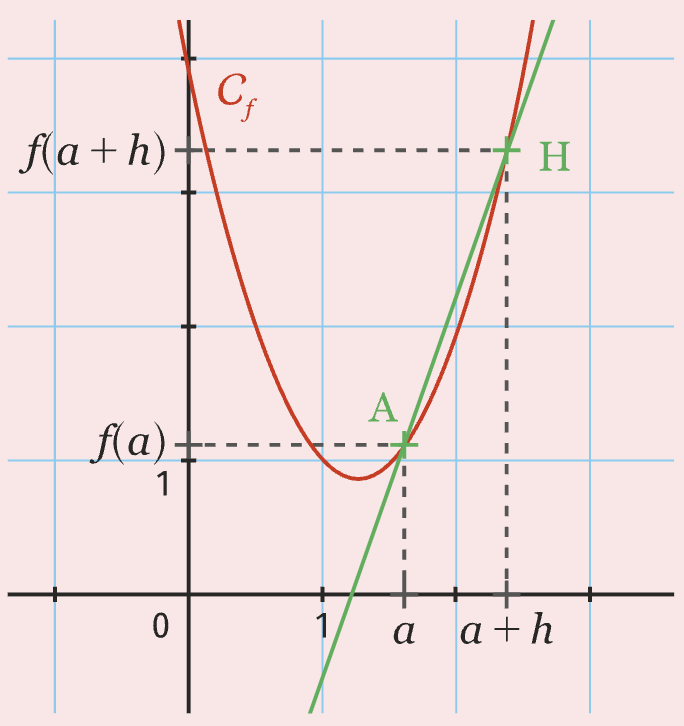
\includegraphics[width=0.95\textwidth]{graphdef.png}
\end{minipage}%

\begin{mdframed}[
    linewidth=1pt,
    roundcorner=5pt,
    linecolor=ForestGreen,
    innertopmargin=10pt,
    innerbottommargin=10pt
]
{\color{ForestGreen}\textbf{\underline{Définition :} Nombre dérivé}}

\vspace{5pt}
On dit que $f$ est \textbf{dérivable en a} lorsque $\tau(h)$ tend vers un nombre réel 
quand $h$ prend des valeurs proches de $0$. Ce réel est appelé \textbf{nombre dérivé} 
de $f$ en $a$ et est noté $f'(a)$.

\vspace{5pt}
On écrit alors :
\[
f'(a) = \lim\limits_{h \to 0} \dfrac{f(a+h)-f(a)}{h}
\]
\end{mdframed}

\begin{questions}
    \question On considère la fonction $f$ suivante définie sur $\mathbb{R}$ :
    \[
    f(x) = -\dfrac{1}{3}x + 1
    \]
    \begin{parts}
        \part Soit $h$ un réel non nul. Calculer $f(3+h)$ et $f(3)$.
        \part Montrer que $f$ est dérivable en 3 et déterminer le nombre dérivé de $f$
        en $3$ (que l'on écrit $f'(3)$).
    \end{parts}

    \vspace{5pt}
    \question (Difficile) Montrer que la fonction $g(x) = \sqrt{x}$ n'est pas dérivable en $0$.
\end{questions}

\vspace{5pt}
\it{\underline{Indices : } Pour ces questions, on pourra d'abord calculer puis simplifier le 
calcul du taux de variation, puis ensuite trouver la limite lorsque h se rapproche de 0.

\vspace{5pt}
Lorsque $h$ tend vers 0 (ou se rapproche de 0), il se rapproche si près que l'on peut donner des approximations.
Mais attention à ne pas confondre avec "\textbf{égal} à 0". Si h se retrouve au dénominateur, 
on peut le faire tendre vers 0 car il n'est \textbf{jamais} égal à 0}.

\end{document}
